\chapter{Design}\label{cha:design}
After conducting my review of previous work, an analysis of the high-level design of the solution was conducted, in particular focusing on the following areas:
\begin{itemize}
	\item Required Features
	\item Technologies and Frameworks
	\item Architecture
\end{itemize}

The aim of this process was to ensure that the limited development time for this project was spent developing the most effective features.

\section{MoSCoW Requirements}

Before considering specific technologies and frameworks, a list of MoSCoW requirements is produced. Each requirement in the table below has two extra columns. The first column represents whether the requirement is Functional (F) or Non-Functional (NF), and the second column represents requirements that Must (M), Should (S) or Could (C) be completed.

\begin{center}
	\begin{xltabular}{0.82\paperwidth}{ | p{1.5cm} | p{1.5cm} | X | } 
		\hline
		F / NF& Priority & Requirement Description \\ \hline
		
 		\multicolumn{3}{|c|}{Domain Specific Language - Expressions} \\ \hline
		F & M & The language must support 5 data types: integers, floats, booleans, strings and date-time objects. \\ \hline
		F & M & The language must be able to tolerate null values in the results of a dataset. \\ \hline
		F & M & The language must allow users to reference a field in the current dataset. \\ \hline
		F & M & The language must allow users to reference a constant value, which can take one of the data types defined above. \\ \hline
		F & M & The language must support arithmetic operations like add, subtract, multiply, division and modulo. \\ \hline
		F & M & The language must support string slicing and concatenation. \\ \hline
		F & S & The language should utilise polymorphism in add operations to apply string concatenation, or arithmetic addition depending on the data types of the arguments. \\ \hline
		F & C & The language could be designed in such a way to allow the user to define their own functions. \\ \hline
		NF & S & The language should be intuitive to use, with SQL-like syntax. \\ \hline
		
		\multicolumn{3}{|c|}{Domain Specific Language - Comparisons} \\ \hline
		F & M & The user must be able to provide expressions as inputs to comparison operators. \\ \hline
		F & M & The language must support equals, and not equals comparisons \\ \hline
		F & M & The language must support inequalities, using numerical ordering for number types, and lexicographic ordering for strings. \\ \hline
		F & M & The language must support null and not null checks. \\ \hline
		F & S & The language should support string comparisons, including case sensitive and insensitive versions of contains, starts with, and ends with. \\ \hline
		F & S & The language should allow the user to combine multiple comparison criteria using $AND$ and $OR$ operators. \\ \hline
		
		\multicolumn{3}{|c|}{Data Processing} \\ \hline
		F & M & The system must allow the user to write queries in Python. \\ \hline
		F & M & The system must allow users to apply Select operations on datasets, applying custom expressions to the input data. \\ \hline
		F & M & The system must allow users to apply Filter operations on datasets, applying custom comparisons to the input data. \\ \hline
		F & M & The system must allow users to apply Group By operations on datasets, which take a number of expressions as unique keys, and a number of aggregate. \\ \hline
		F & M & The Group By operation must allow users to apply Minimum, Maximum, Sum and Count aggregate functions to Group By operations. \\ \hline
		F & C & The system could allow users to apply Distinct Count, String Aggregate, and Distinct String Aggregate aggregate functions to Group By operations. \\ \hline
		F & S & The system should allow users to join two datasets together according to custom criteria. \\ \hline
		NF & S & The complexities of the system should be hidden from the user; from their perspective the operation should be identical whether the user is running the code locally or over a cluster. \\ \hline
		
		\multicolumn{3}{|c|}{Cluster} \\ \hline
		F & M & The system must allow the user to upload source data to a permanent data store. \\ \hline
		F & M & The orchestrator node must split up the full query and delegate partial work to the worker nodes. \\ \hline
		F & M & The orchestrator node must collect partial results from the cluster nodes to produce the overall result for the user. \\ \hline
		F & M & The orchestrator node must handle worker node failures and other computation errors by reporting them to the user. \\ \hline
		F & S & The orchestrator should perform load balancing to ensure work is evenly distributed among all nodes. \\ \hline
		F & C & The orchestrator could handle worker node failures by redistributing work to active workers. \\ \hline
		F & M & The worker nodes must accept partial work, compute and return results to the orchestrator. \\ \hline
		F & M & The worker nodes must pull source data from the permanent data store. \\ \hline
		F & M & The worker nodes must report any computation errors to the orchestrator. \\ \hline
		F & S & The worker nodes should cache results for reuse in later queries. \\ \hline
		F & S & The worker nodes should spill data to disk storage when available memory is low. \\ \hline
	\end{xltabular}
\end{center}

\section{Language}

\subsection{Frontend} 
Python \todo{Reference} was selected as the language of choice for the frontend. This is because the intended users of my solution are most experienced with Python and SQL, which should make adopting the solution faster and easier.
\todo{Expand upon this choice}

\subsection{Orchestrator and Worker Nodes}
Both the orchestrator and worker nodes would use the same language, which would reduce overhead as the same codebase could be used for both parts of the system. When selecting a language, a decision had to be made to use a language with either automatic or manual garbage collection (GC). Choosing a manually GC language would theoretically allow for higher  performance due to more granular control over memory allocation and release. However, this could result in slower development, as time would have to be spent writing code to perform this process. Therefore, manually GC languages were ruled out.

The remaining options were a range of object-oriented and functional languages. Due to the nature of the project, much of the implementation would be CPU intensive, requiring iterating over large lists of items, so a language with strong support for parallelisation was preferable. Functional languages are strong at this because of their use of operations like $map$ and $reduce$, which can be easily parallelised. This also ruled out languages like Python \todo{Reference} and JavaScript \todo{Reference} which are largely single-threaded \todo{Reference}; both support some form of parallelisation, but much more manual intervention by the developer is required.

In the end, Scala was chosen\todo{Reference}. It features a mix of both object-oriented, and functional paradigms, The mix of programming paradigms would allow for the best option to be selected for each task to be completed. Scala has built-in support for parallelised operations and threading through the use of asynchronous operations like Futures and Promises \todo{Reference}. Furthermore, it is built on top of, and compiles into Java. This means that packages originally written for Java can be executed in Scala \todo{Reference}, which proved useful for later design decisions.
 
\section{Runtime}
\subsection{Containerisation}
With the nature of the project being to produce a distributed system, the clear choice for executing the code was within containers. Docker \todo{Reference} is by far the most popular option for creating images to run as containers, but is not suitable for running and managing large numbers of containers \todo{Reference}. For this, a container orchestration tool is required, and there are two main options: Docker Swarm \todo{Reference}, and Kubernetes \todo{Reference}. Docker Swarm is more closely integrated within the Docker ecosystem, and can be managed directly from Docker Desktop. However, Kubernetes is more widely used in industry \todo{Reference} and many cloud services also feature  managed Kubernetes services which handle the complexity of creating and managing a cluster. For this reason, Kubernetes was chosen for the container orchestration tool.

\subsection{Network Communication} 
A communication method had to be selected to allow the Python frontend, the orchestrator and the worker nodes to communicate. REST API frameworks initially appeared to be a suitable option, but upon further research, remote procedure call (RPC) frameworks would be more suited to the project's needs. This is because REST is resource-centric, providing a standard set of operations - create, read, update, delete (CRUD) \todo{Reference}. The proposed solution is more focused on operations than acting on resources, so the CRUD model wouldn't fit the requirements correctly. 

In contrast, RPC frameworks are designed to allow function calls over a remote network, while hiding the complexity of the communication from the developer \todo{reference}. They are also typically not designed around a particular data model like REST, which would allow custom function calls to  be implemented \todo{Reference}. 

The chosen framework was gRPC \todo{Reference}, which is designed and maintained by Google. Firstly, there are well-maintained implementations for both Python and Scala, which would make using it in all parts of the solution straightforward \todo{reference}. Secondly, it uses protocol buffers (protobuf) \todo{Reference} as its message system, which is a serialisation format also maintained by Google. Protocol buffers are designed to be extremely space efficient, reducing network overhead compared to a solution that used something like XML or JSON \todo{reference}. As protocol buffers are also a serialisation format, APIs are provided to store messages on disk.


\section{Persistent Storage}
There are a wide range of options for persistent data storage. The first key decision in this area was whether to design a custom solution, or use an existing solution. A custom implementation would come with the benefit of being more closely integrated with the rest of the system, but at the cost of increased development time. A decision was made not to create a custom solution due to time constraints, and the amount of work required to achieve this. A number of types of existing file systems and databases were considered, that were not selected for use in the system:
\begin{itemize}
	\item Single System SQL Databases \textit{(Microsoft SQL Server, PostgreSQL, MySQL \todo{Reference 3})}: while this option would be fastest to start using due to extensive   usage in industry, the database would quickly become a bottleneck, as the rate at which data can be read from the server would determine how quickly computations could be performed.
	\item Distributed File Systems \textit{(Hadoop Distributed File System \todo{Reference})}: these provide a mechanism for storing files resiliently across a number of machines, which would reduce the bottleneck when reading data. However, they provide no straightforward way of querying the stored data, so this feature would have to be implemented manually.
	\item Distributed NoSQL Databases \textit{(MongoDB, CouchDB \todo{Reference 2})}: these are distributed, meaning the load of reading the data could be spread across a number of machines. However, the input data is tabular, meaning the features of a NoSQL architecture are not required. This is likely to result in added complexity when retrieving data from the database, and increased development time.
\end{itemize}

\subsection{Apache Cassandra} 
In the end, Apache Cassandra \todo{Reference} was chosen for persistent storage. This has a number of benefits for the proposed solution. Firstly, the data model is tabular, and as such closely matches the format of the expected input data. Furthermore, Cassandra is a distributed database, so source data will be stored across a number of nodes, each on different computers. This will increase the effective read speed when retrieving data from the database, as the full load will be spread across all nodes.

\paragraph{Partitioning} Cassandra's method of partitioning data is another key reason why it was selected. Each node in the database is assigned a token range, which determines what records it holds. When data is inserted into the database, Cassandra hashes the primary key of each record, producing a 64-bit token that maps it to a node. A diagram showing this process is included below:
% This should be clear and detailed, it's important
\missingfigure{Cassandra Hashing Process}

Cassandra allows token ranges to be provided as filters in queries, which will allow the worker nodes to control what data is retrieved in each query.

\paragraph{Kubernetes Support} Cassandra can be run on Kubernetes using K8ssandra \cite{k8ssandra}. This is a tool which can be used to initialise, configure and manage Cassandra clusters. This is particularly useful because the Cassandra cluster can be configured to run on the same machines as the worker nodes, enabling the source data to be co-located with the workers that will actually perform the computation, reducing network latency when transferring the source data.

\paragraph{Language-Specific Drivers} In terms of interfacing with the rest of the system, there are drivers for both Python and Java \todo{Reference}, which are maintained by one of the largest contributors to Apache Cassandra. The Java driver has a core module which provides basic functionality for making queries and receiving results from the database. There are optional modules for these drivers with more complex functionality including query builders, but these were not included in the solution as the extra functionality was not required, and the added complexity had the potential to cause problems. 

There are also some Scala specific frameworks for executing Cassandra queries, including Phantom and Quill \todo{Reference}. For the same reason as the optional modules above, these were not chosen for the system.

\section{Architecture}

Based on the above design choices, a high level diagram was produced, detailing each of the components of the system and the interaction between them. 

\begin{figure}[h]
	\centering
	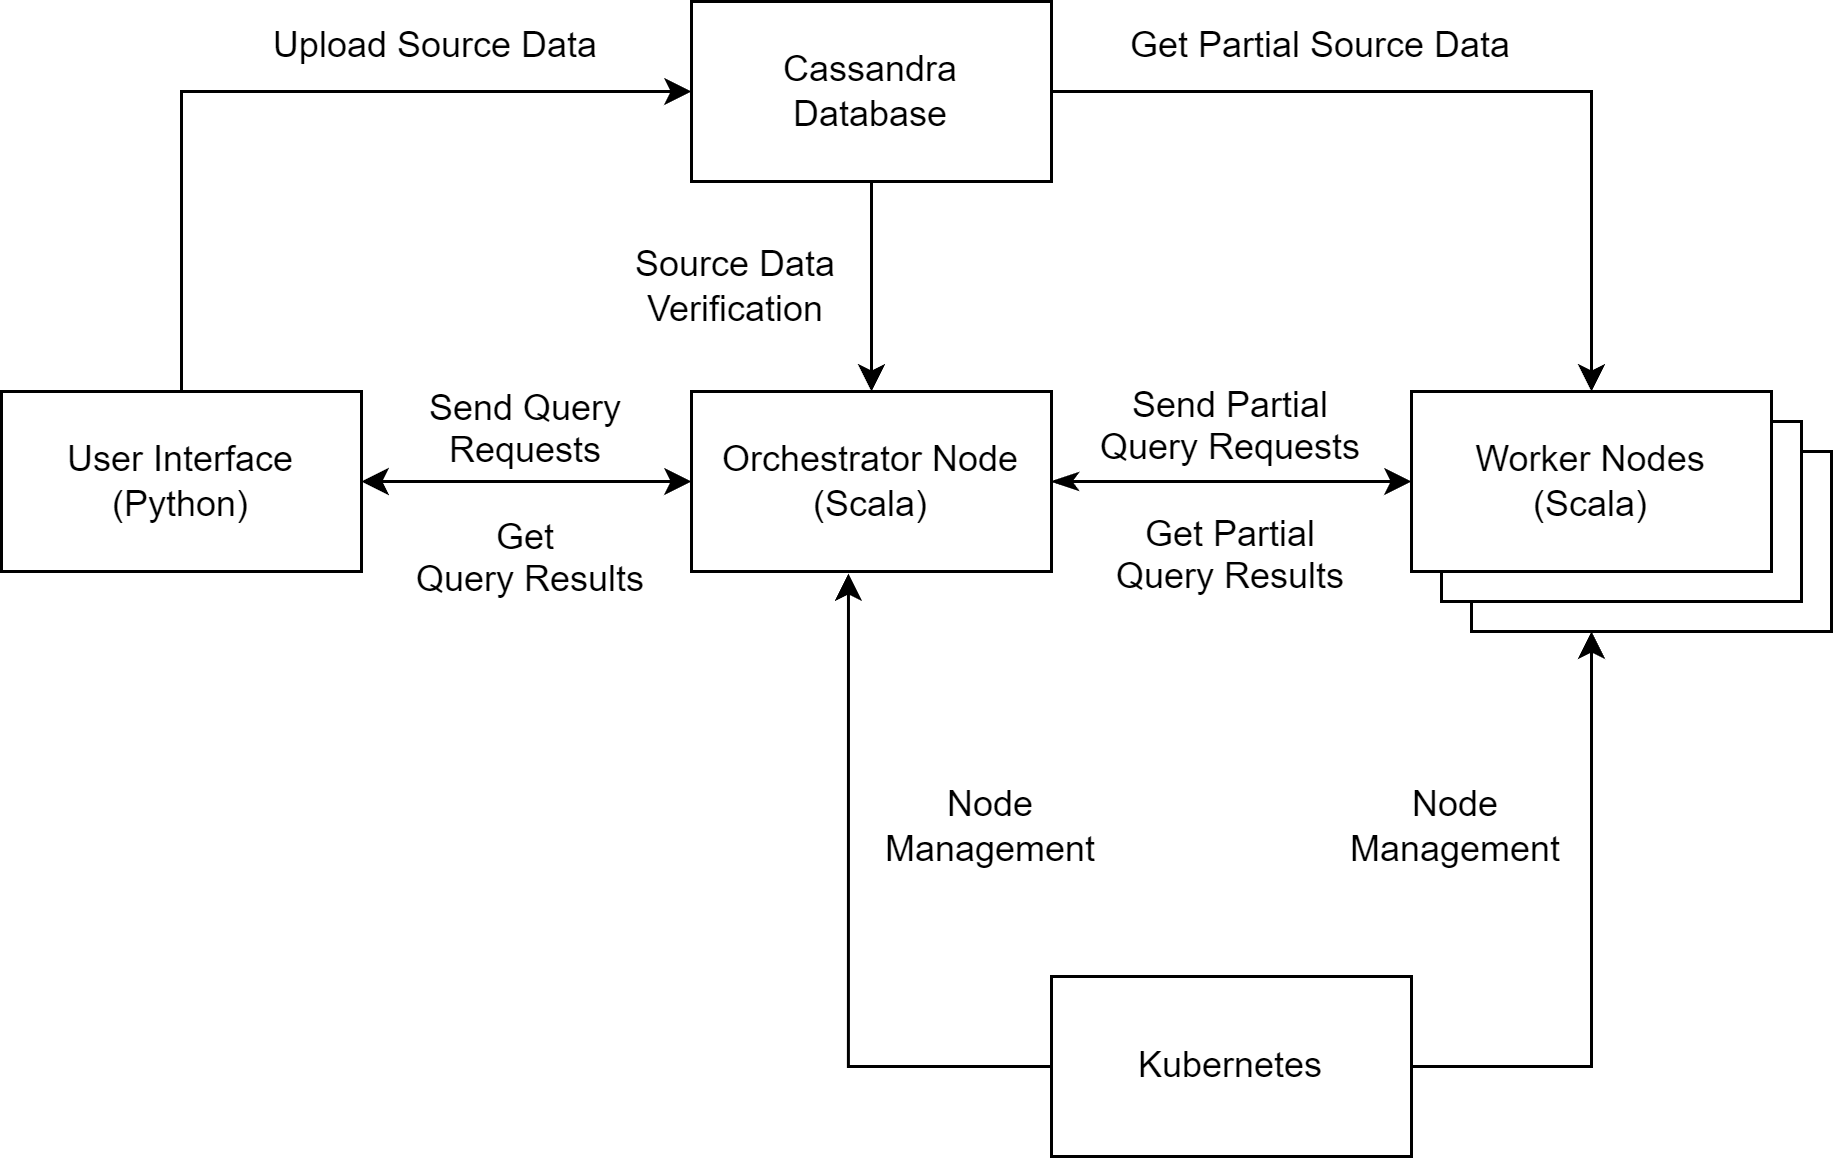
\includegraphics[width=0.5\textwidth]{chapters/diagrams/design/architecture-overall}
	\caption{Overall Architecture Diagram for the Proposed Solution}
\end{figure}

